% =====================================================================
% Chapter 3 -- Theoretical Background
%
% Outline: outlines/ch3_background.md (decisions 2026-10-22).
% Scope: concepts as published, with citations. Own design: Ch. 5; values: Ch. 6.
% Facts: paper_notes/{voxtell,zscl,cpe_clip,lora_hu,liu2026_vlm_cl_survey}.md.
% Notation: thesis_notes.md §5.
% CLAUDE-DRAFT markers removed 2026-11-12 at the author's request; record of the drafted paragraphs: reviews/claude_draft_record.md
% =====================================================================

\chapter{Theoretical Background}
\label{chap:background}

This chapter introduces the concepts on which \cref{chap:method} builds.
\Cref{sec:bg-segmentation} describes volumetric segmentation networks, attention, and the free-text promptable model VoxTell.
\Cref{sec:bg-cl} states the continual-learning problem in the notation used throughout the thesis and describes the published methods from which our strategies are adapted.
\Cref{sec:bg-metrics} defines the evaluation matrix and the metrics with which we measure adaptation and forgetting.

% ---------------------------------------------------------------------
\section{Free-Text Promptable Volumetric Segmentation}
\label{sec:bg-segmentation}

We consider the segmentation of one target structure in a 3D image volume.
A single-channel volume $\mat{X}$ assigns an intensity to every voxel~$v$ of its voxel set~$\Omega$, and the label mask $\mat{Y}$ assigns $y_v = 1$ to the voxels of the structure and $y_v = 0$ to all others.
For this structure, a segmentation network predicts one logit $z_v$ per voxel.
The logistic function~$\sigma$ turns each logit into a foreground probability $\hat{y}_v = \sigma(z_v)$, and thresholding these probabilities gives the binary prediction~$\hat{\mat{Y}}$.
In a free-text promptable model, a text prompt~$p$ names the target structure, so the structure is not tied to a fixed output channel of the network.
One network with parameters~$\theta$ then serves all target structures and computes the logit map $\mat{Z} = f_\theta(\mat{X}, p)$ with entries~$z_v$.
We write $\mathcal{L}_{\mathrm{seg}}$ for the segmentation loss that compares $\mat{Z}$ with $\mat{Y}$.

VoxTell implements $f_\theta$ with a volumetric encoder--decoder network and attention between the text prompt and the image features.

\subsection{Encoder--Decoder Networks for Volumetric Segmentation}
\label{subsec:bg-unet}

The 3D U-Net~\cite{3d_unet} is an encoder--decoder network for volumetric segmentation.
Its encoder computes features at successively lower resolutions in a sequence of stages, and its decoder upsamples them back to the input resolution.
Skip connections pass the encoder features of every stage to the decoder stage of the same resolution, so the decoder can use spatial detail that was lost by downsampling.
We write $\mat{F}_s$ for the encoder features of stage~$s$ and $C_s$ for their number of channels, with $s = 0$ at the full resolution and larger~$s$ at coarser resolutions.
The authors of VoxTell regard this design as still the strongest architecture for 3D medical image segmentation~\cite[Sec.~3]{rokuss2025voxtellfreetextpromptableuniversal}.

A whole volume and its intermediate features often do not fit into the memory of a GPU, so volumetric segmentation networks are trained on patches cut from the volumes.
At inference, a sliding window applies the network to overlapping patches, and their predictions are combined into one prediction per volume.
The nnU-Net framework configures these steps automatically for a given dataset~\cite{isensee2018nnunetselfadaptingframeworkunetbased}.

\subsection{Attention}
\label{subsec:bg-attention}

Attention lets each of a set of query vectors collect information from a set of source vectors, weighting each source by how well it matches the query~\cite{NIPS2017_3f5ee243}.
Let the rows of $\mat{U} \in \mathbb{R}^{n_q \times d}$ be $n_q$ query vectors and the rows of $\mat{S} \in \mathbb{R}^{n_s \times d}$ be $n_s$ source vectors of dimension~$d$.
Multi-head attention projects the query vectors to queries with a learned matrix $\mat{W}_q \in \mathbb{R}^{d \times d}$ and the source vectors to keys and values with $\mat{W}_k, \mat{W}_v \in \mathbb{R}^{d \times d}$, and it splits each projection into $n_h$ heads of dimension $d_h = d / n_h$.
We write all projections as maps $\vec{x} \mapsto \mat{W}\vec{x}$ of column vectors, so they appear transposed when applied to the row-wise inputs $\mat{U}$ and~$\mat{S}$.
Let $\mat{W}_q^{(i)}, \mat{W}_k^{(i)}, \mat{W}_v^{(i)} \in \mathbb{R}^{d_h \times d}$ denote the rows of the projection matrices that belong to head~$i$.
Head~$i$ and the output of multi-head attention are then
\begin{equation}
\begin{aligned}
\operatorname{head}_i &= \operatorname{softmax}\!\left( \frac{\mat{U}\mat{W}_q^{(i)\top} \big(\mat{S}\mat{W}_k^{(i)\top}\big)^{\!\top}}{\sqrt{d_h}} \right) \mat{S}\mat{W}_v^{(i)\top},\\
\operatorname{MHA}(\mat{U}, \mat{S}) &= \big[\operatorname{head}_1, \dots, \operatorname{head}_{n_h}\big]\, \mat{W}_o^{\top},
\end{aligned}
\label{eq:bg-attention}
\end{equation}
where the softmax is taken over the $n_s$ sources for each query, $[\cdot]$ concatenates the heads along the feature dimension, and $\mat{W}_o \in \mathbb{R}^{d \times d}$ is the output projection.
Each query vector thus receives a weighted mean of the values, and the weights are given by the similarity of its query to every key.
The result does not depend on the order of the sources, so a positional encoding is usually added to them.

In self-attention, the query vectors and the source vectors are the same ($\mat{S} = \mat{U}$).
In cross-attention, they come from different inputs, for example a text embedding and image features.
Keys and values are computed from each source vector separately, so further rows appended to~$\mat{S}$ give every query additional sources to attend to without any change to the projections.
The prompt-tuning strategy (\cref{subsec:method-prompt}) relies on this property.

A transformer decoder layer combines attention blocks with a feed-forward network, two linear layers with a nonlinearity between them that are applied to every query separately~\cite{NIPS2017_3f5ee243}.
Each block is wrapped in a residual connection and a layer normalisation.
In the original transformer, each decoder layer applies self-attention to its queries and then cross-attention to the output of the transformer encoder.

\subsection{VoxTell}
\label{subsec:bg-voxtell}

VoxTell is a vision--language model that maps a 3D volume and a free-text prompt to a segmentation mask of the structure that the prompt describes.
The text prompt can range from a single word to a clinical sentence.
The model has four parts (\cref{fig:ch3_voxtell}): a frozen text encoder, a convolutional image encoder, a transformer prompt decoder that relates the text to the image, and a convolutional decoder into which the text is fused at every resolution~\cite[Secs.~1, 3, and~5]{rokuss2025voxtellfreetextpromptableuniversal}.
\Cref{sec:method-adaptation} describes where the version used in this thesis differs from the paper.

\begin{figure}[tb]
\centering
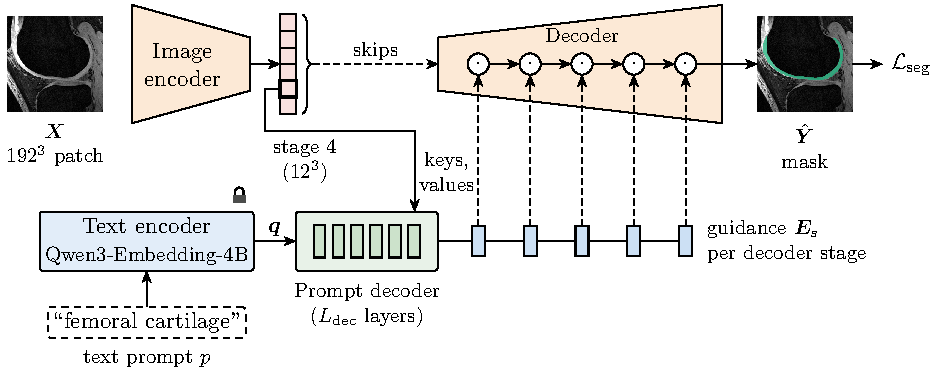
\includegraphics{figures/ch3_voxtell.pdf}
\caption[Architecture of VoxTell]{Architecture of VoxTell (adapted from~\cite[Fig.~2]{rokuss2025voxtellfreetextpromptableuniversal}).
Each of the six stages of the image encoder passes its features to the decoder at the same resolution (skips).
The text encoder embeds the text prompt into the query~$\vec{q}$ and is frozen (lock).
In the prompt decoder, $\vec{q}$ attends to the bottleneck features.
The output of the prompt decoder is mapped to a text-guidance matrix~$\mat{E}_s$ for each of the five decoder stages and fused into that stage (circles, \cref{eq:bg-voxtell-fusion}).
The input is a knee \gls{mri} patch from SKM-TEA with the text prompt ``femoral cartilage''.
For illustration, the output shows the reference mask, not a prediction.}
\label{fig:ch3_voxtell}
\end{figure}

VoxTell is built on the nnU-Net framework~\cite[Suppl.~Sec.~A]{rokuss2025voxtellfreetextpromptableuniversal}, and its image encoder is the residual encoder of the nnU-Net configuration ResEnc~L~\cite[Sec.~3.1]{isensee2024nnunetrevisited}.
The encoder has six stages ($s = 0, \dots, 5$) with 32, 64, 128, 256, 320, and 320 channels~\cite[Suppl.~Sec.~A.2]{rokuss2025voxtellfreetextpromptableuniversal}.
For a patch of $192^3$ voxels, the coarsest stage has $6^3$ voxels.
The text encoder is the embedding model Qwen3-Embedding-4B~\cite{zhang2025qwen3embedding}, which maps the text prompt~$p$ to an embedding $\vec{q} = f_{\mathrm{text}}(p)$~\cite[Eq.~2]{rokuss2025voxtellfreetextpromptableuniversal}.
Before encoding, a fixed instruction is placed in front of the text prompt.
The instruction asks the encoder to retrieve the anatomical entity and location that the text prompt describes~\cite[Suppl.~Sec.~A.2]{rokuss2025voxtellfreetextpromptableuniversal}.
The text encoder is frozen, so the parameters~$\theta$ of VoxTell comprise all parameters except those of~$f_{\mathrm{text}}$.

The prompt decoder consists of $L_{\mathrm{dec}} = 6$ transformer decoder layers of the kind described in \cref{subsec:bg-attention}, with eight heads and dimension $d = 2048$~\cite[Sec.~3, Eq.~3, Suppl.~Sec.~A.2]{rokuss2025voxtellfreetextpromptableuniversal}.
Its query is the text embedding~$\vec{q}$, and its keys and values are the features~$\mat{F}_5$ of the coarsest stage, the bottleneck.
For each decoder stage~$s$, a two-layer perceptron maps the output of the prompt decoder to a text-guidance matrix $\mat{E}_s \in \mathbb{R}^{G \times C_s}$.
Its $G = 32$ rows are guidance vectors of dimension~$C_s$.
The guidance depends on both the text prompt and the image, because the query attends to the image features before it is mapped to the guidance.

The decoder upsamples the features stage by stage and fuses the guidance into every stage~\cite[Eqs.~4--6]{rokuss2025voxtellfreetextpromptableuniversal}.
Starting from $\mat{H}_5 = \mat{F}_5$, it computes for $s = 4, \dots, 1$
\begin{equation}
\mat{H}'_s = \operatorname{ConvBlock}\big(\big[\operatorname{Up}(\mat{H}_{s+1});\, \mat{F}_s\big]\big),
\qquad
\mat{H}_s = \big[\mat{H}'_s;\, \mat{E}_s \odot \mat{H}'_s\big],
\label{eq:bg-voxtell-fusion}
\end{equation}
where $\operatorname{Up}$ upsamples to the resolution of stage~$s$, $\operatorname{ConvBlock}$ denotes the convolutional layers of a decoder stage, $[\cdot\,;\cdot]$ concatenates along the channel dimension, and $\mat{E}_s \odot \mat{H}'_s$ denotes the $G$ maps of dot products between each guidance vector and the $C_s$-dimensional feature vector at every voxel.
Each map thus shows how well the features at every voxel match one guidance vector, and the $G$ maps enter all following convolutions as additional channels.
At the full resolution, $s = 0$, the decoder features are combined with the guidance once more to give the output logits~$\mat{Z}$.

VoxTell was trained with a combination of the binary cross-entropy and the Dice loss~\cite[Sec.~3, Eq.~7, Suppl.~Sec.~A.3]{rokuss2025voxtellfreetextpromptableuniversal}.
With deep supervision, the loss was applied to the outputs of all five decoder stages, with weights from 1 at the full resolution down to $1/16$ as in nnU-Net.
Training used patches of $192^3$ voxels, of which 85\,\% were sampled to contain foreground.
It used the data augmentation of nnU-Net without left--right mirroring.
The optimiser was \gls{sgd} with an initial learning rate of $10^{-4}$ and polynomial decay.
Each training image was paired with three text prompts, two naming structures present in the image and one naming an absent structure, so that the model also learns to return an empty mask.
Each text prompt was the default name of its concept with probability 0.25 and a rephrased variant otherwise.

% ---------------------------------------------------------------------
\section{Continual Learning}
\label{sec:bg-cl}
% Scope (decided 2026-10-22, revised 2026-10-27; restructured 2026-10-29): the problem in symbols,
% the scenario definitions (3.2.1), then the published methods
% the strategies build on (3.2.2-3.2.4; replay only in Ch. 5.4.3, removed 2026-10-30). Evaluation matrix: Sec. 3.3. Classification of our setting
% Ch. 5.1 (moved 2026-10-30); use of the task identity by task-specific LoRA: Ch. 5.4.2 (2026-10-31).
% Informal concepts: Ch. 1; method families: Ch. 2.

This section states the continual-learning problem in the notation of this thesis and defines three common continual-learning scenarios.
It then describes the published methods on which our strategies are based, as they were originally proposed.
These are low-rank adaptation, knowledge distillation with ZSCL, and prompt learning with CoCoOp and CPE-CLIP.
\Cref{sec:method-strategies} presents the corresponding strategies and explains how we adapted these methods to VoxTell and where our versions differ from the originals.

\subsection{Problem Setting and Scenarios}
\label{subsec:bg-cl-setting}

In continual learning, a model is trained on a sequence of tasks $t = 1, \dots, T$, one after the other.
Training on task~$t$ starts from the parameters $\theta_{t-1}$ reached after the previous task, uses only the training data $\mathcal{D}_t^{\mathrm{tr}}$ of task~$t$, and yields the parameters~$\theta_t$.
In our setting, the sequence starts from the pretrained parameters~$\theta_0$, and each task has its own text prompt~$p_t$.
We index the resulting models by the stage~$j$ of the sequence: stage $j = 0$ is the pretrained model, and stage $j = t$ is the model after training on task~$t$.

Van de Ven et al.\ distinguish three continual-learning scenarios by whether the task identity of an input is given at inference and, if it is not, whether the model has to determine it~\cite{van_de_Ven_2025}.
In task-incremental learning, the task identity is given at inference.
In domain-incremental learning, the possible outputs stay the same while the input data changes, and the model is not told the domain of an input.
In class-incremental learning, the model has to distinguish all classes seen so far, including classes it never saw together in training, and thereby also has to infer the task.

\subsection{Low-Rank Adaptation}
\label{subsec:bg-lora}

\Gls{lora} keeps a pretrained weight matrix $\mat{W}_0 \in \mathbb{R}^{d_{\mathrm{out}} \times d_{\mathrm{in}}}$ frozen and learns an additive update of low rank~\cite[Sec.~4.1]{hu2022lora},
\begin{equation}
\mat{W} = \mat{W}_0 + \gamma_r \, \mat{B}\mat{A},
\qquad \mat{B} \in \mathbb{R}^{d_{\mathrm{out}} \times r}, \quad \mat{A} \in \mathbb{R}^{r \times d_{\mathrm{in}}}, \quad r \ll \min(d_{\mathrm{in}}, d_{\mathrm{out}}),
\label{eq:bg-lora}
\end{equation}
where only $\mat{A}$ and $\mat{B}$ are trained and $\gamma_r$ is a scaling factor.
$\mat{A}$ is initialised randomly and $\mat{B}$ with zeros, so the update is zero at the start and training begins from the pretrained model.
After training, $\gamma_r\mat{B}\mat{A}$ can be added to $\mat{W}_0$, so the adapted model has no additional inference cost, and switching to another task only requires exchanging the update.
Hu et al.\ applied LoRA to the projection matrices of self-attention (\cref{eq:bg-attention}).
Comparing choices under a fixed number of trainable parameters, they found that adapting the query and value projections together gave the best performance overall~\cite[Secs.~4.2 and~7.1, Table~5]{hu2022lora}.

In the original formulation, the scaling factor is $\alpha / r$ with a constant hyperparameter~$\alpha$~\cite[Sec.~4.1]{hu2022lora}.
Kalajdzievski showed that this factor makes the gradients of the adapter collapse as the rank grows, so that large ranks learn no better than small ones.
The paper also proves that, in the limit of large rank, only a factor of order $1/\sqrt{r}$ keeps the outputs and gradients of the adapter stable~\cite[Secs.~2.1 and~3]{kalajdzievski2023rankstabilizationscalingfactor}.
The resulting rank-stabilised LoRA (rsLoRA) sets
\begin{equation}
\gamma_r = \frac{\alpha}{\sqrt{r}}.
\label{eq:bg-rslora}
\end{equation}
In fine-tuning experiments with a large language model and ranks up to 2048, rsLoRA improved with increasing rank while standard LoRA did not, and the gradient norms showed the same pattern with \gls{sgd} as with AdamW~\cite[Sec.~4]{kalajdzievski2023rankstabilizationscalingfactor}.

\subsection{Knowledge Distillation and ZSCL}
\label{subsec:bg-zscl}

In knowledge distillation, a student model is trained to reproduce the output distribution of a teacher model, where a temperature in the softmax softens the distribution~\cite[Sec.~2]{hinton2015distilling}.
In continual learning, distillation serves as a regulariser.
Learning without Forgetting (LwF) trains on the data of the new task only and uses the outputs of the model before this task as soft labels for the earlier tasks~\cite{li2017learningforgetting}.
The teacher is thus the previous model, and the distillation data are those of the current task.

ZSCL changes two choices of LwF to preserve CLIP's zero-shot transfer during continual learning~\cite[Sec.~3.2, Eqs.~2--4]{zheng2023preventingzeroshottransferdegradation}.
The teacher is the initial pretrained model instead of the previous one, and the distillation data are a separate reference dataset of unlabelled public images and arbitrary texts instead of the current task's data.
For each image, a softmax turns CLIP's similarities to a set of texts into a distribution, and the loss compares the distributions of student and teacher by a cross-entropy.
A second term does the same for each text, with a distribution over the images of a batch, and both terms are added to the task loss with a weight~$\lambda$.
ZSCL also limits the change of the parameters themselves.
The full method adds a weight-consolidation loss, a penalty on the squared distance between the parameters and a reference set of parameters~\cite[Sec.~3.3, Eq.~5, Table~2]{zheng2023preventingzeroshottransferdegradation}.
Every $I_{\mathrm{we}}$ iterations, it also updates a weight ensemble, the running mean of the parameters along the training trajectory, starting from $\theta_0$,
\begin{equation}
\hat{\theta}_\nu = \frac{1}{\nu+1}\,\theta + \frac{\nu}{\nu+1}\,\hat{\theta}_{\nu-1}, \qquad \hat{\theta}_0 = \theta_0,
\label{eq:bg-we}
\end{equation}
where $\theta$ are the current parameters and $\nu$ counts the ensemble updates~\cite[Sec.~3.3, Eq.~7]{zheng2023preventingzeroshottransferdegradation}.

\subsection{Prompt Learning and CPE-CLIP}
\label{subsec:bg-prompt}

Prompt learning adapts a frozen vision--language model by training a few input vectors instead of its weights.
CoOp replaces the hand-written context words of a text prompt, such as ``a photo of a'', by learnable context vectors in front of the class name~\cite{zhou2022coop}.
CoCoOp adds a small network, the meta-net, which computes a token from the image features and adds it to every context vector, so that the context vectors depend on the input image~\cite[Secs.~3.3 and~4.1]{zhou2022cocoop}.
Its authors report that these image-dependent context vectors generalise better to classes not seen in training.

CPE-CLIP applies prompt learning to few-shot class-incremental learning~\cite[Secs.~1 and~3]{D_Alessandro_2023}.
In this setting, a base session with many classes and examples is followed by sessions that each add a few classes with few examples, and the task identity is not given at evaluation~\cite[Secs.~2.3 and~3]{D_Alessandro_2023}.
CPE-CLIP keeps CLIP frozen and learns prompt tokens in the layers of the language encoder up to a given depth, where each layer replaces the prompt tokens it receives by its own learned ones~\cite[Sec.~4, Eqs.~2--4]{D_Alessandro_2023}.
The prompt tokens of the vision encoder are derived from those of the language encoder by a learned linear projection~\cite[Sec.~4, Eqs.~6--8]{D_Alessandro_2023}.
To limit forgetting, CPE-CLIP scales the gradients of the prompt tokens and of the projection in session~$t$ by
\begin{equation}
\beta_t = \frac{|\mathcal{C}_t|}{\sum_{\tau=0}^{t} |\mathcal{C}_\tau|},
\label{eq:bg-cpe-scaling}
\end{equation}
where $\mathcal{C}_t$ is the set of classes of session~$t$, so that the prompt tokens change less as more classes have been learned~\cite[Sec.~4, Eqs.~11--13]{D_Alessandro_2023}.

% ---------------------------------------------------------------------
\section{Evaluation Metrics}
\label{sec:bg-metrics}
% Definitions as implemented in scripts/compute_cl_metrics.py (reference implementation).
% Which metrics are reported and why: Ch. 6 setup (decision 2026-10-21).

This section defines the segmentation metric and the continual-learning metrics computed from it.

The overlap between a binary prediction $\hat{\mat{Y}}$ and the label mask $\mat{Y}$ is measured with the \gls{dsc}~\cite{dice1945measures},
\begin{equation}
\operatorname{DSC}(\hat{\mat{Y}}, \mat{Y}) = \frac{2\,|\hat{\mat{Y}} \cap \mat{Y}|}{|\hat{\mat{Y}}| + |\mat{Y}|},
\label{eq:bg-dsc}
\end{equation}
where $|\cdot|$ counts the foreground voxels of a mask and $\hat{\mat{Y}} \cap \mat{Y}$ denotes the voxels that are foreground in both.
The \gls{dsc} is 0 for disjoint masks and 1 for identical ones.
The \gls{dsc} is normalised by the sizes of the two masks and not by the size of the volume, so the many background voxels do not inflate it.
This matters for structures as small as the knee cartilages and menisci (\cref{sec:data-skmtea}).

Evaluating the model on every task after every stage shows how training on later tasks affects earlier ones~\cite[Fig.~4b]{zheng2023preventingzeroshottransferdegradation}.
We write $a_{i,j}$ for the mean \gls{dsc} on the test set of task~$i$ after stage~$j$, with $i = 1, \dots, T$ and $j = 0, \dots, T$.
Together, the values $a_{i,j}$ form the evaluation matrix.
The forgetting and intransigence measures of Chaudhry et al.\ were originally defined for classification accuracy, but the authors note that a task-specific measure such as the \gls{iou} of a segmentation can take the place of accuracy without changing the definitions~\cite[Sec.~3]{Chaudhry_2018}.
The diagonal entries $a_{i,i}$ show how well task~$i$ is learned when it is trained.
The entries with $j > i$ show how much of this performance is kept after later tasks, and the entries with $j < i$ show the performance on task~$i$ before it is trained.
Entries $a_{i,j} < a_{i,i}$ with $j > i$ therefore indicate catastrophic forgetting of task~$i$.
The matrix does not show whether the model loses pretrained abilities outside the task sequence, because its rows cover only the tasks of the sequence.
We measure this loss of pretrained ability with a control task, a held-out task that is never trained on.
We write $c_j$ for its mean \gls{dsc} after stage~$j$.

\begin{figure}[tb]
\centering
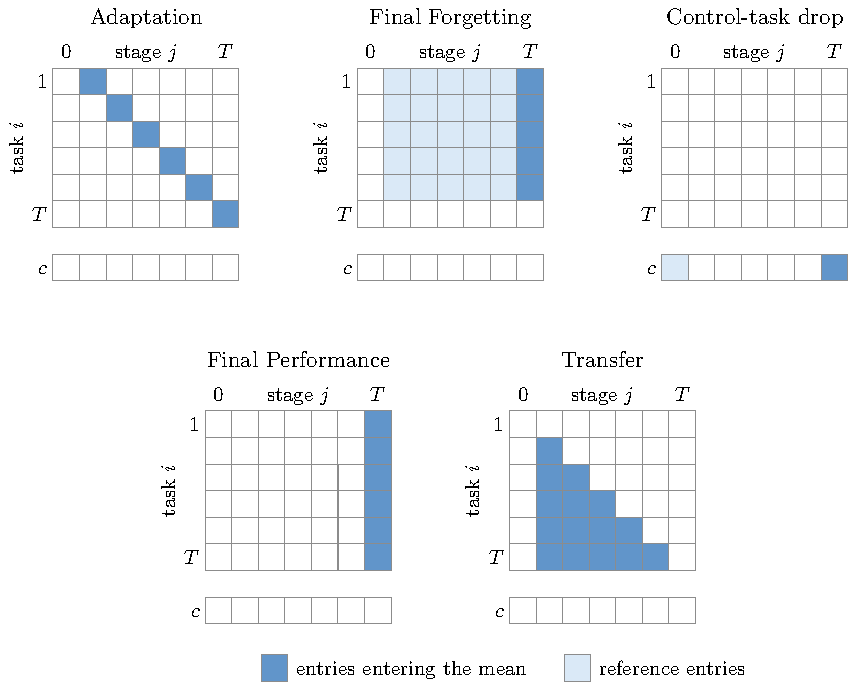
\includegraphics{figures/ch3_metrics.pdf}
\caption[Entries of the evaluation matrix used by each metric]{Entries of the evaluation matrix used by each metric.
Rows are the tasks $i = 1, \dots, T$, and columns are the stages $j = 0, \dots, T$, with stage~0 the pretrained model.
The separate row~$c$ is the control task.
Dark cells enter the mean of a metric.
Light cells are the reference from which the dark cell of the same row is subtracted, namely their maximum for Final Forgetting and the pretrained value $c_0$ for the control-task drop.}
\label{fig:ch3_metrics}
\end{figure}

We summarise the evaluation matrix with four metrics, three taken from the literature and one derived from it, and the control task with a fifth.
\Cref{fig:ch3_metrics} shows which entries each metric uses.

\paragraph{Adaptation.}
Adaptation measures how well each task is learned when it is trained,
\begin{equation}
\text{Adaptation} = \frac{1}{T} \sum_{i=1}^{T} a_{i,i}.
\label{eq:bg-adaptation}
\end{equation}
Each diagonal entry $a_{i,i}$ also appears in the intransigence measure of Chaudhry et al.
This measure subtracts it from the performance on task~$i$ of a reference model trained on the data of tasks $1, \dots, i$ together~\cite[Sec.~3, Eq.~4]{Chaudhry_2018}.

\paragraph{Final Forgetting.}
Final Forgetting is the average forgetting of Chaudhry et al.\ after the last task~\cite[Sec.~3, Eq.~3]{Chaudhry_2018}.
For each task before the last, it subtracts the performance at the end from the best performance at any stage from 1 to $T-1$,
\begin{equation}
\text{Final Forgetting} = \frac{1}{T-1} \sum_{i=1}^{T-1} \Big( \max_{j \in \{1, \dots, T-1\}} a_{i,j} - a_{i,T} \Big).
\label{eq:bg-forgetting}
\end{equation}
Taking the best earlier performance instead of the value right after training also counts gains that a task made while later tasks were trained and lost again by the end.
Lower values are better, and a negative value means that training on later tasks improved earlier ones, which Chaudhry et al.\ call positive backward transfer.

\paragraph{Control-task drop.}
The control-task drop follows SPU, which uses a control set to measure how much of a pretrained model's general ability is lost during continual learning~\cite[Sec.~5.1, Eq.~6]{Zhang_2024_CVPR}.
SPU computes this loss as the accuracy of the frozen pretrained model on the control set minus that of the continually trained model.
We compute the drop with the \gls{dsc}, between the pretrained model and the model after the last stage of a task sequence,
\begin{equation}
\text{Control-task drop} = c_0 - c_T,
\label{eq:bg-control-drop}
\end{equation}
so a positive value is a loss and lower values are better.

\paragraph{Final Performance.}
Final Performance is the metric Last of ZSCL, the mean performance on all tasks after the last stage~\cite[Sec.~4, Fig.~4b]{zheng2023preventingzeroshottransferdegradation},
\begin{equation}
\text{Final Performance} = \frac{1}{T} \sum_{i=1}^{T} a_{i,T}.
\label{eq:bg-final}
\end{equation}
A common reference for Final Performance is joint training, in which one model is trained on the data of all tasks at once.
De Lange et al.\ describe joint training as a soft upper bound for continual learning~\cite[Sec.~6.2.1]{delange2022}.

\paragraph{Transfer.}
Transfer is the metric of the same name in ZSCL~\cite[Sec.~4, Fig.~4b]{zheng2023preventingzeroshottransferdegradation}.
For each task~$i$, it averages the performance at the stages $1, \dots, i-1$ before the task is trained, and it then averages these values over the tasks,
\begin{equation}
\text{Transfer} = \frac{1}{T-1} \sum_{i=2}^{T} \frac{1}{i-1} \sum_{j=1}^{i-1} a_{i,j}.
\label{eq:bg-transfer}
\end{equation}
Stage $j = 0$ is not included, as in ZSCL, whose evaluation matrix has no entries for the model before the first training step.
The first task therefore does not enter Transfer.
When the task sequence starts from a pretrained model, as here, an entry $a_{i,j}$ with $j < i$ reflects both the ability of the pretrained model on structure~$i$ and the effect of training on tasks $1, \dots, j$.
Transfer does not separate the two.
The pretrained-model reference row (\cref{sec:method-setting-protocol}) shows the first part alone.

